\chapter{Project Background}
\label{chap:antecedentes}


This chapter resumes the main subjects acquired during the accomplishment of the GEO-Cloud project.  The novel architecture proposed in this project for EO processing carries the absence of this kind of platforms to compare with. In this way, the study of the state of the art will be done focalising in some aspects of cloud computing platforms, federated testbeds, networking, satellite systems, and so on. As consequence, this section depicts the different thematic areas .
The conceptual map showed in Figure~\ref{fig:intr-conceptual-map} presents the sections and subsections of this chapter. Thereby in Earth Observation Satellites area, the different concepts for creating and modelling a satellite for earth imaging, its data management and orbital definitions is studied. In high-level languages, some scripting languages are compared. In Networking section, different network impairments and several tools for acquiring these are depicted. In Federated Infrastructre section, the testbeds that Fed4FIRE platform is composed by are explained.

\begin{figure}[!h]
\begin{center}
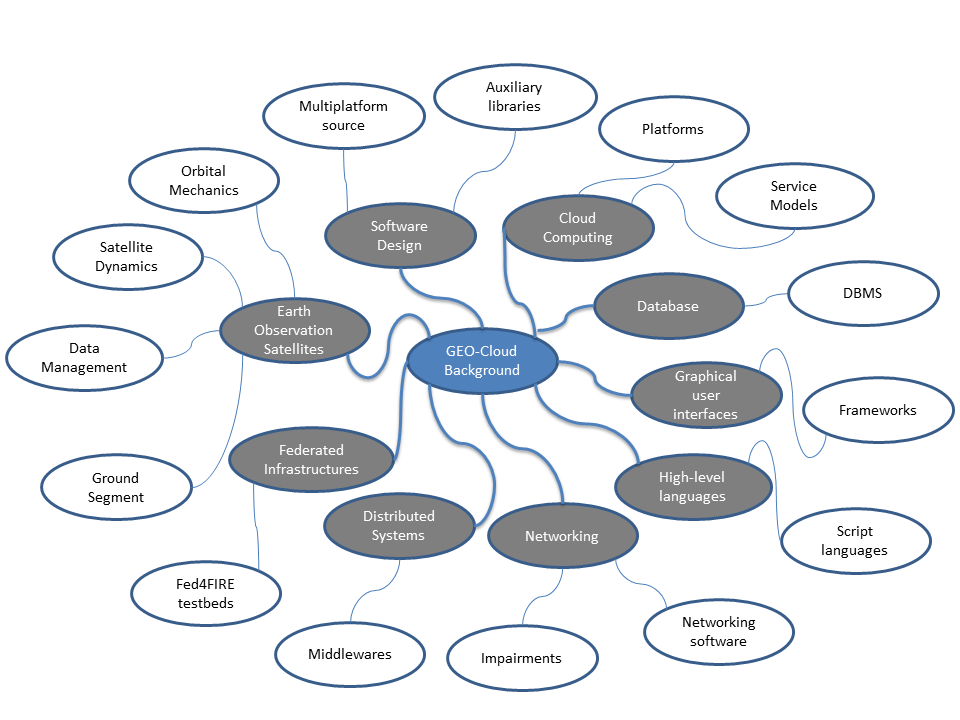
\includegraphics[width=1\textwidth]{statement/background-geocloud.png}
\caption{Conceptual Map of this chapter.}
\label{fig:intr-conceptual-map}
\end{center}
\end{figure}

In the section explains the Graphical User Interfaces background, several
frameworks for developing GUIs are depicted. In Database section, differents
database management systems are compared. The distributed systems section
explains and compares some middlewares as Hadoop or ZeroC Ice for developing
distributed applications.
Finally, in the Software Design section discusses the requirements for building multiplatform code, and other ancillary libraries required by the detailed objectives of GEO-Cloud.

\section{Earth Observation Satellites}

In this section, different areas of aeronautics are involved. The orbital
mechanics which defines and calculates the satellite orbits for rounding around
the world; the Satellite Dynamics whose aim consist of defining the main
features of the satellite and payloads to carry out a concrete mission; and
finally, the data management whose mission consist of storing and sending the
usefull information from satellite to Ground Segment.

\subsection{Orbital Mechanics}

\subsection{Satellite Dynamics}

\subsection{Data Management}


\section{High-level languages}

For the development of the project, \acs{XML}, Python and Bash languages has
been used. The first, XML, has been used for building the configuration file of
the Orchestrator component and to obtain the selected nodes by JFed
application. The rest of them are scripting languages. The source of the
components of the cloud has been developed using Python and the interconnections
between modules and others secundary funcionalities, in Bash script.

\subsection{XML}
\acs{XML} is a markup language that defines a set of rules for encoding
documents in a format that is both human-readable and machine-readable. Most of
actual software use it for configuring or for updating its configuration on fly.

\subsection{Python}
Python is a object oriented language, although permits imperative and functional
programming. It does not need to compile the source because it is
interpreted. It permits a flexible development because it is dynamic type and in
this project, the most important feature why this language has been used,
consist of it is multiplatform. With this feature, the software is able to be
executed in any platform. The current version is 2.7.4 and it offers several
useful and multipourpose libraries as matlib, pthread, mysqllib, pdb and so on.

\subsection{Bash Script}

It consists of several sentences that the operative system is able to read and
translate in order to play a determined action. All the currents Linux
distributions contains a Bash interpret
\section{Networking}
\section{Federated Infrastructures}
\section{Graphical User Interfaces}

\section{Database}

\section{Distributed Systems}

\section{Software Design}


\section{Estilos de texto}

Debido a su continuo uso, se muestra entre paréntesis la combinación del modo
\texttt{auctex} de GNU Emacs para incluir el comando \LaTeX{} correspondiente.

\begin{itemize}
\item Normal.
\item \textbf{Negrita} (C-c-f-b).
\item \textit{Itálica} (C-c-f-i).
\item \emph{Enfatizada} (C-c-f-e). Fíjate que el estilo que se obtiene al
  enfatizar depende del estilo del texto en el que se incluya: \textit{texto en
    itálica y \emph{enfatizado} en medio}.
\item \texttt{Monoespaciada} (C-c-f-t)
\end{itemize}

Otros de menos uso:

\begin{itemize}
\item \textsc{Versalita} (C-c-f-c).
\item \textsf{Serifa}, es decir, sin remates o paloseco (C-c-f-f).
\item \textrm{Romana} (C-c-f-r).
\end{itemize}


\section{Viñetas y enumerados}

En \LaTeX{} hay tres tipos básicos de viñetas:

\begin{itemize}
\item itemize.
\item enumerate.
\item description.
\end{itemize}


Es posible hacer viñetas (como la siguiente) cambiando márgenes u otras
propiedades gracias al paquete \href{http://mirror.ctan.org/macros/latex/contrib/enumitem/enumitem.pdf}{\emph{enumitem}}
(ya incluido en \arcopfc).

\begin{itemize}[noitemsep, label=$\triangleright$]
\item esto es
\item una pequeña
\item muestra
\end{itemize}

El paquete \emph{enumitem} ofrece muchas otras posibilidades para personalizar
las viñetas (individual o globalmente) o crear nuevas.


\section{Figuras}

Las figuras se referencian así (ver figura~\ref{fig:informatica}). Recuerda que
no tienen porqué aparecer en el lugar donde se ponen (mira un libro de
verdad). \LaTeX{} las colocará donde mejor queden, No te empeñes en
contradecirle, él sabe mucho de tipografía.

\begin{figure}[!h]
\begin{center}
\includegraphics[width=0.2\textwidth]{/informatica.pdf}
\caption{Escudo oficial de informática}
\label{fig:informatica}
\end{center}
\end{figure}

Por cierto, los títulos de tablas, figuras y otro elementos flotantes (los
\texttt{caption}) no deben acabar en punto~\cite{sousa}.


\section{Cuadros}
\label{sec:uncuadro}

Se denominan «tablas» cuando contienen datos con relaciones numéricas. En
general se denominan «cuadros». Si las columnas están bien alineadas, las líneas
verticales estorban más que ayudan (no las pongas). Los cuadros se referencian
de este modo (ver cuadro~\ref{tab:rpc-semantics}).

\begin{table}[hp]
  \centering
  {\small
  


\begin{tabular}{p{.2\textwidth}p{.2\textwidth}p{.2\textwidth}p{.2\textwidth}}
  \tabheadformat
  \tabhead{Tipo de fallo}   &
  \tabhead{Sin fallos}      &
  \tabhead{Mensaje perdido} &
  \tabhead{Servidor caído}  \\
\hline
\textit{Maybe}         & Ejecuta:   1 & Ejecuta: 0/1        & Ejecuta: 0/1 \\
                       & Resultado: 1 & Resultado: 0        & Resultado: 0 \\
\hline
\textit{Al-least-once} & Ejecuta:   1 & Ejecuta:   $\geq$ 1 & Ejecuta:   $\geq$ 0 \\
                       & Resultado: 1 & Resultado: $\geq$ 1 & Resultado: $\geq$ 0 \\
\hline
\textit{At-most-once}  & Ejecuta:   1 & Ejecuta:   1        & Ejecuta: 0/1 \\
                       & Resultado: 1 & Resultado: 1        & Resultado: 0 \\
\hline
\textit{Exactly-once}  & Ejecuta:   1 & Ejecuta:   1        & Ejecuta:   1 \\
                       & Resultado: 1 & Resultado: 1        & Resultado: 1 \\
\hline
\end{tabular}


% Local variables:
%   coding: utf-8
%   ispell-local-dictionary: "castellano8"
%   TeX-master: "main.tex"
% End:

  }
  \caption[Semánticas de \acs{RPC} en presencia de distintos fallos]
  {Semánticas de \acs{RPC} en presencia de distintos fallos
    (\textsc{Puder}~\cite{puder05:_distr_system_archit})}
  \label{tab:rpc-semantics}
\end{table}


\section{Listados de código}
\label{sec:listado}

Puedes referenciar un listado con~\ref{code:hello}. Éste es un listado flotante,
pero también pueden ser «no flotantes» (mira la documentación del paquete
\href{http://www.ctan.org/get/macros/latex/contrib/listings/listings.pdf}{«listings»}).

\begin{listing}[
  float=ht,
  language = C,
  caption  = {«Hola mundo» en C},
  label    = code:hello]
#include <stdio.h>
int main(int argc, char *argv[]) {
    puts("Hola mundo\n");
}
\end{listing}

Puedes modificar el estilo por defecto para tus listados añadiendo un comando
\texttt{lstset} en tu \texttt{main.tex}. El código LaTeX del listado \ref{code:custom-listings}
añade un fondo gris claro y una línea en el margen izquierdo.

\begin{listing}[
  float=h!,
  caption  = {Personalizando los listados de código},
  label    = code:custom-listings]
\lstset{%
  backgroundcolor = \color{gray95},
  rulesepcolor    = \color{black},
}
\end{listing}



\section{Citas y referencias cruzadas}

Puedes ver aquí una cita~\cite{design_patterns} y una referencia a la segunda sección
(véase \S\,\ref{sec:uncuadro}). Para hacer referencias debes definir etiquetas en el punto
que quieras referenciar (normalmente justo debajo). Es útil que los nombres de las
etiquetas (comando label) tengan los siguientes prefijos (incluyendo los dos puntos ``:''
del final):

\begin{description}
\item[chap:] para los capítulos. Ej: ``\texttt{chap:objetivos}''.
\item[sec:] para secciones, subsecciones, etc.
\item[fig:] para las figuras.
\item[tab:] para las tablas.
\item[code:] para los listados de código.
\end{description}

Si estás viendo la versión PDF de este documento puedes pinchar la cita o el número de
sección. Son hiper-enlaces que llevan al elemento correspondiente. Todos los elementos que
hacen referencia a otra cosa (figuras, tablas, listados, secciones, capítulos, citas,
páginas web, etc.) son «pinchables» gracias al paquete
\href{http://latex.tugraz.at/_media/docs/hyperref.pdf}{\emph{hyperref}}.

Para citar páginas web usa el comando \texttt{url} como en: \url{http://www.uclm.es}

\section{Páginas}
\label{sec:paginas}

La normativa dice que el documento debería ser impreso a una cara, pero si el
número de páginas es alto puede imprimirse a dos caras. Como eso es bastante
subjetivo, mi consejo es que ronde las 100 \textbf{hojas}. Es decir, si el
documento tiene más de 200 páginas imprímelo a doble cara, si tiene menos
imprímelo a una.

Por defecto, \arcopfc{} imprime a una cara (oneside), si quieres imprimir a doble cara,
escribe en el preámbulo:

\begin{listing}
  \documentclass[twoside]{arco-pfc}
\end{listing}

Esto es importante porque a doble cara los márgenes son simétricos y a una cara
no. Si llevas el PFC a la copistería y pides que te lo impriman de modo
diferente al generado, quedará mal ¡Cuidado!
